\documentclass[12pt]{article}
\usepackage[utf8]{inputenc}
\usepackage[T1]{fontenc}
\usepackage{fontspec}
\setmainfont{Times New Roman}
\newfontfamily\hackfont{Hack}
\usepackage{titlesec}
\usepackage{fancyhdr}
\usepackage{listings}
\usepackage{xcolor}
\usepackage{graphicx}
\usepackage{longtable}
\usepackage{caption}
\usepackage{hyperref}
\usepackage{setspace}
\usepackage{geometry}
\usepackage{array}
\usepackage{longtable}
\geometry{a4paper, margin=1in}
\hypersetup{colorlinks=true, linkcolor=blue, urlcolor=blue}

\pagestyle{fancy}
\fancyhf{} 							% Header Middle
\rhead{Computer Networks Lab Final}
\lhead{VLSM Design}
\rfoot{\thepage}

\begin{document}

\begin{titlepage}					% Cover Start
\begin{center}
    
\includegraphics[width=0.35\textwidth]{logo.png} \\
    \vspace{0.5cm}
    \textbf{\Huge \textcolor{teal}{NOTRE DAME} \textcolor{teal}{UNIVERSITY}} \\
    \vspace{0.5cm}
    \textbf{\Huge \textcolor{orange}{BANGLADESH}} \\
    
    \vspace{0.9cm}
    \textbf{\Huge \underline{Computer Networks Lab Final}} \\
    
    \vspace{1.5em}
    \begin{flushleft}
    	\textbf{\Large Course Code: CSE-3204} \\
		\vspace{0.3cm}        
        \textbf{\Large Course Title: Computer Networks Lab} \\
        \vspace{0.3cm}
        \textbf{\Large Lab Final Task : VLSM Design for 172.05.0.0/16 Network} \\        
    \end{flushleft}
    
    \vspace{1em}
    \begin{flushleft}
        \textbf{\Huge \textcolor{blue}{Submitted by:}} \\
        \vspace{0.3cm}
        \textbf{\Large Name: Istiak Alam} \\
        \vspace{0.3cm}
        \textbf{\Large ID: 0692230005101005} \\
		\vspace{0.3cm}        
        \textbf{\Large Batch: CSE-20} \\
        \vspace{0.5cm}
        \textbf{\Large Submission Date: }{\Large \textbf{\today}\par}
    \end{flushleft}
    \vfill
    \begin{flushleft}
        \textbf{\Huge \textcolor{blue}{Submitted to:}} \\
        \vspace{0.3cm}
        \textbf{\Large Dr. Fernaz Narin Nur} \\
        \vspace{0.3cm}
        \textbf{\Large Adjunct Professor,} \\
        \vspace{0.3cm}
        \textbf{\Large Notre Dame University Bangladesh}
    \end{flushleft}
\end{center}
\end{titlepage}						% Cover End


\section*{Objective}
To implement and understand the working of \textbf{VLSM Design for 172.05.0.0/16 Network} using Cisco Packet Tracer, Optimize IP Address Utilization: Different departments (CSE, EECE, ICT, SH, Admin T) require different numbers of hosts.VLSM allows us to assign subnets based on actual need (e.g., 2000 hosts for CSE, only 125 for Admin T). This avoids wasting IP addresses compared to using a fixed-size subnet for all.

\section*{VLSM Table for 172.05.0.0/16}

\begin{longtable}{|>{\bfseries}m{2.5cm}|m{1.8cm}|m{1cm}|m{3cm}|m{3cm}|m{3.5cm}|}
\hline
Network Name & Hosts Required & CIDR & Subnet Mask & Network Address & Usable IP Range \\
\hline
CSE & 2000 & /21 & 255.255.248.0 & 172.05.0.0 -- 172.05.7.255 & 172.05.0.1 -- 172.05.7.254 \\
ECE & 1000 & /22 & 255.255.252.0 & 172.05.8.0 -- 172.05.11.255 & 172.05.8.1 -- 172.05.11.254 \\
ICT & 500  & /23 & 255.255.254.0 & 172.05.12.0 -- 172.05.13.255 & 172.05.12.1 -- 172.05.13.254 \\
SH  & 200  & /24 & 255.255.255.0 & 172.05.14.0 -- 172.05.14.255 & 172.05.14.1 -- 172.05.14.254 \\
Admin T & 125 & /25 & 255.255.255.128 & 172.05.15.0 -- 172.05.15.127 & 172.05.15.1 -- 172.05.15.126 \\
\hline
\end{longtable}

\section*{Router-to-Router Links (\texttt{/30} subnets)}
\begin{itemize}
  \item N1--N2: \texttt{172.05.16.0/30} $\rightarrow$ \texttt{172.05.16.1 -- 172.05.16.2}
  \item N1--N3: \texttt{172.05.16.4/30} $\rightarrow$ \texttt{172.05.16.5 -- 172.05.16.6}
  \item N1--N4: \texttt{172.05.16.8/30} $\rightarrow$ \texttt{172.05.16.9 -- 172.05.16.10}
  \item N2--CSE: \texttt{172.05.16.12/30} $\rightarrow$ \texttt{172.05.16.13 -- 172.05.16.14}
  \item N3--ECE: \texttt{172.05.16.16/30} $\rightarrow$ \texttt{172.05.16.17 -- 172.05.16.18}
  \item N4--ICT: \texttt{172.05.16.20/30} $\rightarrow$ \texttt{172.05.16.21 -- 172.05.16.22}
  \item N3--SH: \texttt{172.05.16.24/30} $\rightarrow$ \texttt{172.05.16.25 -- 172.05.16.26}
  \item N4--AdminT: \texttt{172.05.16.28/30} $\rightarrow$ \texttt{172.05.16.29 -- 172.05.16.30}
\end{itemize}
\newpage
\section*{Network Topology}
\begin{figure}[h!]
    \centering
    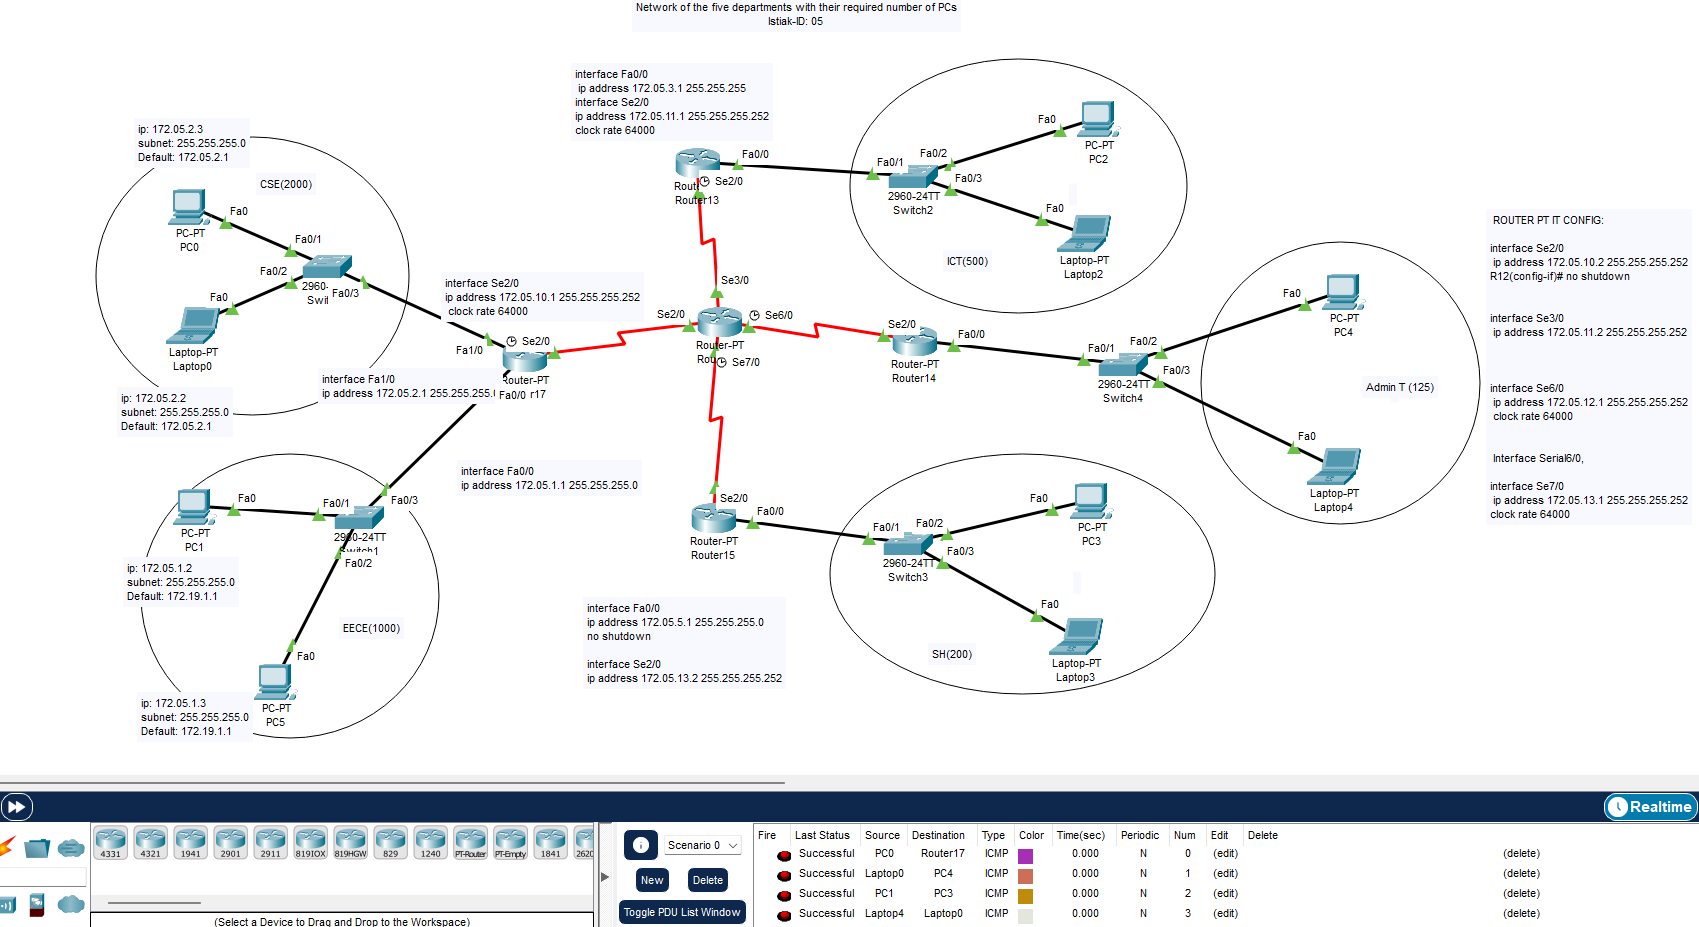
\includegraphics[width=1\linewidth]{ss.png}
    \caption{Topology}
    \label{fig:enter-label}
\end{figure}

\section*{Router Configuration :}

\subsection*{Router N1}
\begin{lstlisting}[basicstyle=\ttfamily\small, frame=single]
hostname N1
interface GigabitEthernet0/0
 ip address 172.05.16.1 255.255.255.252
 no shutdown
interface GigabitEthernet0/1
 ip address 172.05.16.5 255.255.255.252
 no shutdown
interface GigabitEthernet0/2
 ip address 172.05.16.9 255.255.255.252
 no shutdown
exit
ip routing
\end{lstlisting}
\newpage
\subsection*{Router N2}
\begin{lstlisting}[basicstyle=\ttfamily\small, frame=single]
hostname N2
interface GigabitEthernet0/0
 ip address 172.05.16.2 255.255.255.252
 no shutdown
interface GigabitEthernet0/1
 ip address 172.05.16.13 255.255.255.252
 no shutdown
exit
ip routing
\end{lstlisting}

\subsection*{Router N3}
\begin{lstlisting}[basicstyle=\ttfamily\small, frame=single]
hostname N3
interface GigabitEthernet0/0
 ip address 172.05.16.6 255.255.255.252
 no shutdown
interface GigabitEthernet0/1
 ip address 172.05.16.17 255.255.255.252
 no shutdown
interface GigabitEthernet0/2
 ip address 172.05.16.25 255.255.255.252
 no shutdown
exit
ip routing
\end{lstlisting}

\subsection*{Router N4}
\begin{lstlisting}[basicstyle=\ttfamily\small, frame=single]
hostname N4
interface GigabitEthernet0/0
 ip address 172.05.16.10 255.255.255.252
 no shutdown
interface GigabitEthernet0/1
 ip address 172.05.16.21 255.255.255.252
 no shutdown
interface GigabitEthernet0/2
 ip address 172.05.16.29 255.255.255.252
 no shutdown
exit
ip routing
\end{lstlisting}
\newpage
\section*{DHCP Configuration Examples}

\subsection*{CSE}
\begin{lstlisting}[basicstyle=\ttfamily\small, frame=single]
ip dhcp pool CSE
 network 172.05.0.0 255.255.248.0
 default-router 172.05.0.1
 dns-server 8.8.8.8
\end{lstlisting}

\subsection*{ECE}
\begin{lstlisting}[basicstyle=\ttfamily\small, frame=single]
ip dhcp pool ECE
 network 172.05.8.0 255.255.252.0
 default-router 172.05.8.1
 dns-server 8.8.8.8
\end{lstlisting}

\subsection*{ICT}
\begin{lstlisting}[basicstyle=\ttfamily\small, frame=single]
ip dhcp pool ICT
 network 172.05.12.0 255.255.254.0
 default-router 172.05.12.1
 dns-server 8.8.8.8
\end{lstlisting}

\subsection*{SH}
\begin{lstlisting}[basicstyle=\ttfamily\small, frame=single]
ip dhcp pool SH
 network 172.05.14.0 255.255.255.0
 default-router 172.05.14.1
 dns-server 8.8.8.8
\end{lstlisting}

\subsection*{AdminT}
\begin{lstlisting}[basicstyle=\ttfamily\small, frame=single]
ip dhcp pool AdminT
 network 172.05.15.0 255.255.255.128
 default-router 172.25.15.1
 dns-server 8.8.8.8
\end{lstlisting}
\newpage
\section*{Testing}
In Cisco Packet Tracer, after giving packet on PC0 to Router17 \& PC1 to PC3 (etc.) the packet send and recive is successful. 
\begin{figure}[h!]
    \centering
    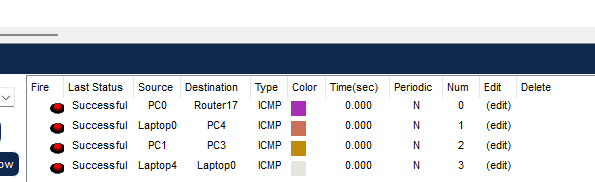
\includegraphics[width=1\linewidth]{image.png}
    \caption{Testing Packets}
    \label{fig:enter-label}
\end{figure}

\end{document}
